\chapter{Аналитический раздел}
\label{cha:analysis}
\section{Цель и задачи работы}
Целью данной работы является создание метода управления памятью в многопоточных приложениях.
Для достижения данной цели необходимо решить следующие задачи:
\begin{itemize}
	\item проанализировать предметную область и существующие методы выделения оперативной памяти приложениям;
	\item разработать метод выделения оперативной памяти приложениям;
	\item создать ПО, тесттирующее различные методы выделения памяти;
	\item создать ПО, реализующее  разработанный метод выделения оперативной памяти.
\end{itemize}

\section{Сложность выделения памяти}

Наименьшая единица адресации памяти в современных операционных системах - страница. Ее размер обычно равен 4КБ, но есть, так называемые, большие   страницы, размер которых варьируется на каждой архитектуре и для x86 состовляет 2МБ. Этот размер ограничен базовым оборудованием. Это означает, что операционная   система не может запросить памяти меньше чем размер страницы. Процессор не умеет работать с памятью   линейно, для получения физического адрес, он делает запрос в УУП (англ. MMU)   (который   по   сутия вляется кешом TLB) и далее уже через него получает нужный адрес. Это тоже своего рода проблема, потому что линейный доступ к памяти обеспечил бы минимум необходимых операций по трансляции виртуальных адресов в физические, но тогда пришлось бы переделывать все что связано с виртуальной памятью   процесса, а значит и переделывать сами процессоры и операционные системы.

Процесс может запросить память у ОС через 2 системных вызова: \textbf{\textit{mmap}} и \textbf{\textit{sbrk}}.

\textbf{\textit{sbrk}} управляет точкой разрыва программы, тоесть функция   опеределяет доступную процессу память просто инкрементируя указатель на свободную память в куче до тех пока, пока не достигнет области отображаемой в процесс памяти.

\textbf{\textit{mmap}} отображает в адресное пространство процесса системные страницы памяти.

Почти все существующие библиотеки отказались от использования \textbf{\textit{sbrk}} в пользу \textbf{\textit{mmap}} по следующим причинам:
\begin{itemize}
	\item у sbrk есть ограничение в виде лимита выделения памяти, данный лимит - это ближайшая к нему отображаемая область памяти;
	\item память выделяется только линейно, нельзя выделить в любом месте кучи как это умеет делать mmap.
\end{itemize}

Вызов \textbf{\textit{mmap}} занимает больше времени, но он более гибок и универсален в использовании. Но одними системными вызовами не получится эффективно управлять оперативной памятью. Каждый системный вызов генерирует прерывание, которое приостанавливает код в пространстве пользователя и перемещается   на исполнение кода в пространстве  ядра, это называется сменой контекста. Смена контекста процесса является тяжелой операцией, которая требует сохранить текущее состояние процесса. Поэтому все библиотеки стараются делать эти вызовы как можно реже и запрашивать у ОС как можно больше памяти за один системный вызов.

\section{TCMalloc}
TCMalloc это аллокатор памяти, разработанный компанией Google и являющийся заменой стандартному системному аллокатору, он имеет следующие характеристики:
\begin{itemize}
	\item Быстрое выделение и освобождение памяти для большинста объектов. Обекты кэшируются в зависимости от режима, либо кэш в каждом потоке, либо кэш на логический процессор. Большинство аллокаций не требуют синхронизации доступа к ресурсам, благодаря этому конкуренция за выделение памяти сводится к минимуму и обеспечивает хорошее масштабирование для многопоточных приложений.
	\item Гибкое использование памяти, освобожденная память может быть переиспользована для объектов различных размеров или возвращена системе.
	\item Низкие накладные расходы на память под каждый объект за счет выделения ``страниц'' объектов одинакового размера. Это позволяет хранить небольшие объекты в памяти эффективно и помогает избежать излишней фрагментации памяти.
	\item Низкая стоимость сэмлирования, которое позволяет получить детальное представление об использовании памяти приложением.
\end{itemize}

\subsection{Общее описание}

\begin{figure}[!h]
	\begin{center}
		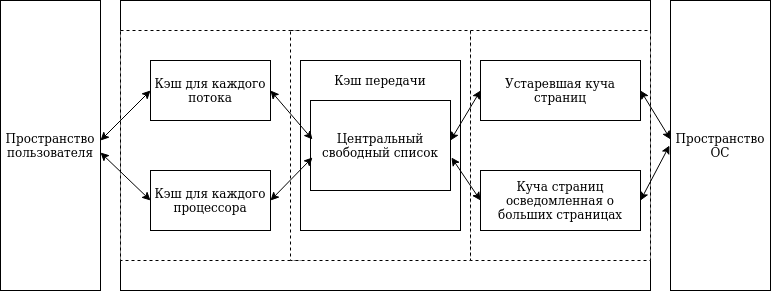
\includegraphics[scale=0.6]{images/tcmalloc-overview.png}
		\caption{Внутренняя структура TCMalloc.}
		\label{tcmalloc-overview}
	\end{center}
\end{figure}

Библиотеку TCMalloc можно разбить на 3 основных компонента. Фронт-энд (англ. front-end), миддл-энд (англ. middle-end) и бэк-энд (англ. back-end):
\begin{itemize}
	\item Фронт-энд является кэшом, который предоставляет быстрое выделение и освобождение памяти приложению.
	\item Миддл-энд отвечает за наполнение фронт-энд кэшей.
	\item Бэк-энд управляет памятью, которая выделяется приложению самой ОС.
\end{itemize}

Фронт-энд может использоваться как в режиме кэш на каждый поток, так и в режиме кэш на каждый логический процессор. Бэк-энд может поддерживать работу с кучей, которая осведомлена о больших страницах.

\subsection{TCMalloc фронт-энд}

Фронт-энд обрабатывает запрос на выделение памяти определенного размера. У него имеется кэш памяти, который может использоваться для выделения или хранения свободной памяти. Этот кэш доступен только одному потоку одновременно, поэтому никаких блокировок не требуется и большинство выделений и освобождений памяти выполняются быстро.

Фронт-энд удовлетворит любой запрос, если у него есть закэшированная память соответствующего размера. Если кэш для этого конкретного размера пуст, будет сделан запрос на пополнение кэша в миддл-энд, который включает в себя центральный список свободной памяти и кэш передачи.

Если миддл-энд исчерпан или запрошенный размер больше максимального размера, который кэшируется фронт-эндом, запрос будет переадресован бек-энду, чтобы либо удовлетворить большое выделение памяти, либо пополнить кэш в миддл-энде. Бэк-энд также называется кучей страниц (англ. pageheap).

На данный момент существует 2 реализации фронт-энда:
\begin{itemize}
	\item Первоначально он поддерживал кэширование объектов по каждому потоку (отсюда и название англ. Thread Caching Malloc). Однако это могло приводить к появлению больних областей памяти, которые масштабировались с увеличением количества потоков. Современные приложения могут иметь большое количество потоков, что приводит либо к большим объемам памяти для каждого потока, либо к тому, что многие потоки имеют крошечные локальные кэши.
	\item Совсем недавно TCMalloc начал поддерживать режим кэширования под каждый логический процессор. В этом режиме каждый процессор в системе имеет свой собственный кэш, из которого выделяется память. Примечание: На x86 логический процессор эквивалентен гиперпотоку.
\end{itemize}

Различия между режимами работы кешей по потокам и процессорам полностью ограничиваются реализациями malloc/new и free/delete.

\subsubsection{Выделение памяти под большие и малые объекты}

Размер на выделение памяти под малые объекты сопоставляется c одним из 60-80 распределяемых размерных классов. Например, выделение 12 байт будет округлено до 16-ти байтового класса размера. Размерные классы предназначены для минимизации объема памяти, который тратится впустую при округлении до следующего по величине размерного класса.

При компиляции с  \_\_STD CPP\_DEFAULT\_NEW\_ALIGNMENT\_\_ <= 8 используется набор размеров, выровненных по 8-ми байтам. Это меньшее выравнивание сводит к минимуму потери памяти для многих распространенных размеров распределения (24, 40 и т.д.), которые в противном случае округляются до кратного 16-ти байтам. Во многих компиляторах это поведение контролируется флагом \textbf{\textit{-fnew-alignment=...}}. Когда \_\_STD CPP\_DEFAULT\_NEW\_ALIGNMENT\_\_ не указан (или больше 8 байт), использются стандартные 16-ти байтовые выравнивания для \textit{\textbf{::operator new}}. Однако при выделении менее 16-ти байт может быть возвращен объект с меньшим выравниванием, так как ни один объект с большим требованием выравнивания не может быть выделен в пространстве.

Когда запрашивается объект заданного размера, запрос сопоставляется с определенным размерным классом с помощью функции \textit{\textbf{SizeMap::GetSizeClass()}}, и возвращаемая память принадлежит этому классу. Это означает, что возвращаемая память по крайней мере так же велика, как и запрошенный размер. Выделения памяти из размерных классов обрабатываются фронт-эндом.

Объекты размером больше предела, определенного максимальным размером (\textbf{kMaxSize}), выделяются непосредственно из бэк-энда. Как таковые они не кэшируются ни фронт ни миддл эндами. Запросы на выделение больших размеров объектов округляются до размера страницы TCMalloc.

\subsubsection{Освобождение памяти}

Когда объект освобождается, компилятор предоставляет размер объекта, если он известен во время компиляции. Если размер не известен, он будет найден на карте страницы. Если объект мал, он будет помещен обратно в кэш фронт-энда. Если объект больше \textbf{\textit{kMaxSize}}, он возвращается непосредственно в кучу страниц.

\subsubsection{Режим кэша под каждый процессор}

В этом режиме выделяется один большой блок памяти. На следующей диаграмме показано как этот блок памяти разделен между процессорами и как каждый процессор использует часть блока для хранения метаданных, а также указателей на доступные объекты.

\begin{figure}[!h]
	\begin{center}
		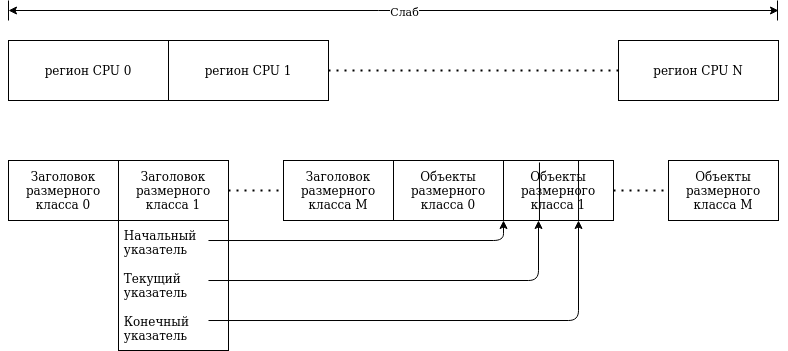
\includegraphics[scale=0.6]{images/tcmalloc-per-cpu.png}
		\caption{Диграмма блока памяти при работе кэша в режиме под каждый процессор.}
		\label{tcmalloc-per-cpu}
	\end{center}
\end{figure}

Каждому логическому процессору назначается секция этой памяти для хранения метаданных и указателей на доступные объекты определенных размерных классов. Метаданные содержат один блок заголовок на каждый размерный класс. Заголовок содержит указатель на начало массива указателей на объекты размерных классов, а также указатель на текущую, динамическую, максимальную емкости и текущую позицию в этом сегменте массива. Статическая максимальная емкость каждого массива указателей для каждого размерного класса определяется во время запуска разницей между началом массива для этого класса и началом массива для следующего класса.

Во время выполнения максимальное количество элементов определенного размерного класса, которое может храниться в блоке для каждого процессора, будет варьироваться, но оно никогда не может превышать статически определенную максимальную емкость, назначенную при запуске.

Когда запрашивается объект определенного размерного класса, он удаляется из этого массива, а когда объект освобождается, он добавляется в массив. Если массив исчерпан, он снова заполняется запросом на выделение памяти в миддл-энд. Если массив переполняется, партия объектов удаляется из него и возвращается в миддл-энд.

Объем памяти, который может быть закэширован, ограничен для каждого процессора параметром \textbf{\textit{MallocExtension::SetMaxPerCpuCacheSize}}. Это означает, что общий объем кэшиуемой памяти зависит от количества активных кэшей под процессоры. Следовательно, машины с более высоким количеством процессоров могут кэшировать больше памяти.

Чтобы избежать удержания памяти на процессорах, где приложение больше не работает, вызывается функция \textbf{\textit{MallocExtension::ReleaseCpuMemory}}, которая освобождает объекты, хранящиеся в кэшах указанного процессора.

Внутри ЦП распределение памяти управляется по всем размерным классам таким образом, чтобы максимальный объем кэшируемой памяти оставался ниже предельно возможного. Тут стоит обратить внимание что он управляет максимальной суммой, которая может быть закэширована, а не суммой, которая в данный момент кэшируется. В среднем, фактически кэшируемая сумма должна составлять примерно половину лимита.

Максимальная емкость увеличивается в тот момент, когда в размерном классе заканчиваются объекты, а также при извлечении большого количества объектов рассматривается возможность увеличения емкости размерного класса. Емкость размерного класса может быть увеличена до тех пор, пока общая память (для всех размерных классов), которую может содержать кэш, не достигнет предела для каждого процессора или пока емкость этого размерного класса не достигнет жестко заданного предела размера для этого размерного класса. Если класс не достиг жестко заданного предела, то для увеличения емкости он может взять емкость из другого размерного класса на том же процессоре.

\subsubsection{Перезапускаемые последовательности и кэш под каждый процессор}

Для правильной работы, режим кэш под каждый процессор опирается на перезапускаемые последовательности (man rseq(2)). Перезапускаемая последовательность - это просто блок инструкций (на языке ассемблера), во многом похожий на типичную функцию. Ограничение перезапускаемых последовательностей состоит в том, что они не могут записывать частичное состояние в память, конечная инструкция должна быть единственной записью обновленного состояния. Идея перезапускаемых последовательностей заключается в том, что если поток удаляется из процессора (например, переключается контекст) во время выполнения перезапускаемой последовательности, то она будет перезапущена сначала. Следовательно, последовательность либо завершится сразу, либо будет многократно перезапущена, пока не завершится без прерываний. Это достигается без использования каких-либо блокирующих или атомарных инструкций, что позволяет избежать конкуренций за ресурсы в самой последовательности.

Практический смысл этого для TCMalloc заключается в том, что код может использовать перезапускаемую последовательность, такую как \textbf{\textit{TcmallocSlab\_Push}}, для извлечения или возврата элемента в массив для каждого процессора без необходимости блокировки. Перезапускаемая последовательность гарантирует, что либо массив обновляется без прерывания потока, либо последовательность перезапускается, если поток был прерван (например, переключателем контекста, который позволяет другому потоку работать на этом процессоре).

\subsubsection{Устаревший режим кэша под каждый поток}

В режиме кэша под каждый поток TCMalloc назначает каждому потоку локальный кэш. Небольшие выделения удовлетворяются из этого локального кэша. Объекты могут перемещаться между миддл-эндом в кэш для потока и из него по мере необходимости.

Потоковый кэш содержит один односвязный список свободных объектов на каждый размерный класс (так что если существует N размерных классов, то будет N соответствующих связных списков), как показано на следующей диаграмме.

\begin{figure}[!h]
	\begin{center}
		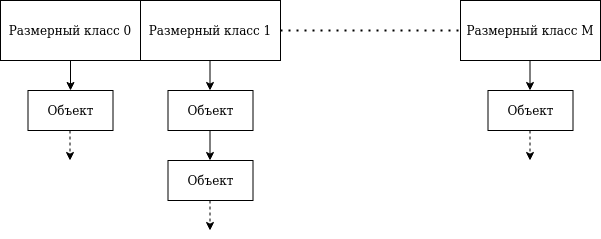
\includegraphics[scale=0.6]{images/tcmalloc-per-thread.png}
		\caption{Диграмма списка свободных объектов при работе кэша в режиме под каждый поток.}
		\label{tcmalloc-per-thread}
	\end{center}
\end{figure}

При выделении объект удаляется из соответствующего размерного класса кэшей для каждого потока. При освобождении объект добавляется к соответствующему списку размерного класса. Переполнение и опустошение обрабатываются путем запроса памяти у миддл-энда или возвращением туда избыточной памяти.

Максимальная емкость кэша для каждого потока устанавливается параметром \textbf{\textit{MallocExtension::SetMaxTotalThreadCacheBytes}}. Однако общий размер может превысить этот предел, так как каждый кэш для каждого потока имеет минимальный размер \textbf{\textit{KMinThreadCacheSize}}, который обычно составляет 512 КБ. В том случае, если поток хочет увеличить емкость своего кэша, ему необходимо уменьшить емкость кэша у других потоков.

По завершению работы потока, вся доступная ему память переходит в миддл-энд в кэш передачи.

\subsection{TCMalloc миддл-энд}

Миддл-энд отвечает за предоставление памяти фронт-энду и возврат памяти в бэк-энд. Он состоит из кэша передачи и центрального свободного списка. Хотя их часто называют сингулярными, существует один кэш передачи и один центральный свободный список на каждый размерный класс. Каждый из этих кэшей защищен мьютексом, поэтому доступ к ним требует затрат на сериализацию.

\subsubsection{Кэш передачи}

Когда фронт-энд запрашивает или возвращает память, он обращается к кэшу передачи. В нем содержится массив указателей на свободную память, и перемещение объектов в этот массив или извлечение объектов из этого массива по запросу фронт-энда происходят быстро.

Кэш передачи получил свое название из ситуаций, когда один поток выделяет память, освобожденную другим потоком. Он позволяет памяти быстро перемещаться между двумя различными потоками. Если кэш передачи не может удовлетворить запрос памяти или имеет недостаточно места для хранения возвращенных объектов, будет совершено обращение к центральному свободному списку.

\subsubsection{Центральный свободный список}

Центральный свободный список управляет памятью в спанах (англ. span), спан или диапазон - это набор из одной или нескольких страниц памяти TCMalloc. Запрос на один или несколько объектов удовлетворяется центральным свободным списком путем извлечения объектов из спанов до тех пор, пока запрос не будет удовлетворен. Если в диапазоне недостаточно доступных объектов, то из бэк-энда запрашиваются дополнительные спаны.

Когда объекты возвращаются в центральный свободный список, каждый объект сопоставляется с областью, к которой он принадлежит (с помощью карты страниц), а затем освобождается в эту область. Если все объекты, находящиеся в определенном диапазоне, возвращаются в него, то весь спан возвращается бэк-энду.

\subsubsection{Карты страниц и спаны}

Куча, управляемая TCMalloc, делится на страницы определенного размера во время компиляции. Область смежных страниц представлена объектом спан. Он может использоваться для управления большим объектом, который был передан приложению, или областью страниц, которые были разделены на последовательность небольших объектов. Если спан управляет малыми объектами, то размерный класс объектов записывается в него.

Карта страниц используется для поиска диапазона, к которому принадлежит объект, или для определения размерного класса для данного объекта. TCMalloc использует 2-ух уровневое или 3-ех уровневое компактное префиксное дерево (англ. radix tree) для отображения всех возможных ячеек памяти на спаны.

На следующей диаграмме показано, как 2-ух уровневая карта страниц используется для отображения адресов объектов на спаны, управляющие системными страницами, в которых находятся объекты. На диаграмме диапазон A занимает две страницы, а диапазон Б 3 страницы.

\begin{figure}[!h]
	\begin{center}
		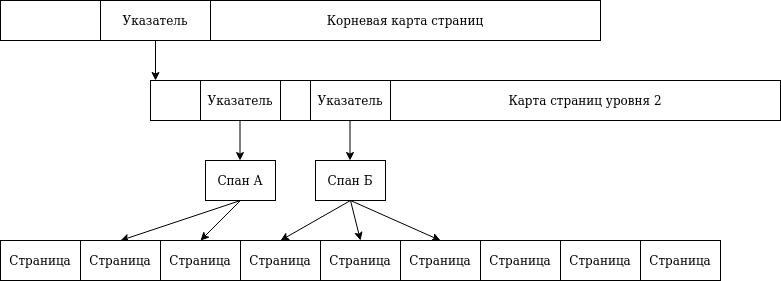
\includegraphics[scale=0.6]{images/tcmalloc-pagemap-and-spans.png}
		\caption{Карта страниц сопоставляет объекты со спанами.}
		\label{tcmalloc-pagemap-and-spans}
	\end{center}
\end{figure}

Спаны используются в миддл-энде для определения места размещения возвращаемых объектов, и в бэк-энде для управления обработкой интервалов страниц.

\subsubsection{Хранение малых объектов в спанах}

Спан содержит указатели на адреса страниц, которыми он управляет. Для небольших объектов эти страницы разделены не более чем на $2^{16}$ объектов. Это значение выбрано таким образом, чтобы в пределах диапазона можно было ссылаться на объекты по двухбайтовому индексу. Это означает, развернутый связный список может быть использован для хранения объектов. Например, если есть 8-ми байтовые объекты, то можно хранить индексы трех готовых к использованию объектов и использовать четвертый слот для хранения индекса следующего объекта в цепочке. Эта структура данных уменьшает пропуски кэша по сравнению с полносвязным списком. Другое преимущество использования двухбайтовых индексов заключается в том, что можно использовать резервную емкость в самом спане для кэширования четырех объектов.

Когда нет доступных объектов определенного размерного класса, необходимо извлечь новый спан из кучи страниц и заполнить его.

\subsubsection{Размеры страниц в TCMalloc}

TCMalloc можно собрать с различными размерами страниц. Тут стоит отметить что они не соответствуют размерам страниц, которое используются в буффере ассоциативной трансляции (англ. TLB) базового оборудования. Эти размеры страниц в настоящее время составляют 4КБ, 8КБ, 32КБ и 256КБ.

Страница TCMalloc либо содержит несколько объектов определенного размера, либо используется как часть группы для хранения объекта размером больше одной страницы. Если вся страница становится свободной, она будет возвращена бек-энду в кучу страниц и позже может быть перепрофилирована для хранения объектов другого размера (или возвращена в ОС).

Небольшие страницы лучше справляются с требованиями приложения к памяти с меньшими накладными расходами. Например, наполовину использованная страница размером в 4КБ будет иметь 2КБ в остатке по сравнению с 32-ух килобайтной страницей, которая будет иметь 16КБ. Маленькие страницы также с большей вероятностью станут свободными. Например, страница в 4КБ может содержать восемь объектов по 512 байт по сравнению с 64-мя объектами на странице размером в 32КБ; и вероятность того, что 32 объекта будут свободны одновременно, намного меньше, чем вероятность того, что восемь станут свободными.

Большие страницы приводят к уменьшению потребности в извлечении и возврате памяти из бэк-энда. Одна страница размером 32КБ может содержать в восемь раз больше объектов, чем страница размером 4КБ, и это может привести к тому, что затраты на управление большими страницами будут меньше. Кроме того, требуется меньше больших страниц для отображения всего виртуального адресного пространства. TCMalloc имеет карту страниц, которая отображает виртуальный адрес на структуры, управляющие объектами в этом диапазоне адресов. Большие страницы означают, что карта страниц нуждается в меньшем количестве записей и, следовательно, она сама меньше.

Исходя из этого, для приложений с небольшими выделениями памяти или чувствительных к размеру областей памяти, имеет смысл использовать меньшие размеры страниц TCMalloc. Приложения с большим объемом памяти, скорее всего, выиграют от увеличения размеров страниц TCMalloc.

\subsection{TCMalloc бэк-энд }

У бэк-энда в TCMalloc есть 3 задачи:
\begin{itemize}
	\item Управление большими диапазонами неиспользуемой памяти.
	\item Извлечение памяти из операционной системы, когда нет подходящего размера памяти, доступной для выполнения запроса на выделение.
	\item Возврат ненужной памяти обратно в ОС.
\end{itemize}

Существует 2 реализации бэк-энда в TCMalloc:
\begin{itemize}
	\item Устаревшая куча страниц, которая управляет памятью в блоках размером со страницу TCMalloc.
	\item Куча страниц, которой известно о больших страницах, она управляет памятью блоками размером с большую страницу (в данном случае речь идет о размере страницы самого базового оборудования). Управление памятью большими страницами позволяет аллокатору повысить производительность приложения за счет уменьшения пропусков в буффере ассоциативной трансляции.
\end{itemize}

\subsubsection{Устаревшая куча страниц}

Устаревшая куча страниц - это массив свободных списков для определенных длин смежных страниц доступной памяти. Для всех индексов меньше 256-ти, список по индексу состоит из диапазонов, размер которых равен индексу умноженному на размер страницы TCMalloc. 256-я запись - это список диапазонов, длина которых >= 256 страниц:

\begin{figure}[!h]
	\begin{center}
		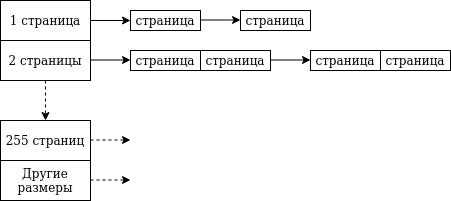
\includegraphics[scale=0.6]{images/tcmalloc-legacy-pageheap.png}
		\caption{Диаграмма устаревшей кучи страниц.}
		\label{tcmalloc-legacy-pageheap}
	\end{center}
\end{figure}

Выделение памяти для N страниц удовлетворяется путем поиска в N-м свободном списке. Если этот свободный список пуст, идет обращение в следующий свободный список и так далее. Если найти нужный диапазон памяти не удается, то память запрашивается у ОС через системный вызов \textbf{\textit{mmap}}.

Если выделение для N страниц удовлетворяется диапазоном страниц длиной большей N, то оставшаяся часть диапазона повторно вставляется обратно в соответствующий свободный список в куче страниц. Когда диапазон страниц возвращается в кучу, соседние страницы проверяются, чтобы определить, образуют ли они теперь непрерывную область, если это так, то страницы объединяются и помещаются в соответствующий свободный список.

\subsubsection{Аллокатор осведомленный о больших страницах}

Главная цель такого аллокатора - держать память в блоках состоящих из больших системных страниц. На архитектуре x86 размер такой страницы равен 2МБ. Для этого в бэк-энде есть 3 разных кэша:
\begin{itemize}
	\item Кэш наполнителя, содержит большие страницы, из которых была выделена некоторая память. Он имеет сходство с устаревшей кучей страниц в том смысле, что содержит связные списки памяти определенного количества страниц TCMalloc. Запросы на выделение ресурсов размером менее чем больщая страница (как правило) возвращаются из кэша наполнителя. Если кэш наполнителя не имеет достаточного количества доступной памяти, он запросит дополнительные большие страницы.
	\item Кэш регионов, который обрабатывает выделения размером более чем размер большой страницы. Данный кэш позволяет выделениям памяти распределяться между несколькими большими страницами и упаковывать несколько таких выделений в непрерывную область. Это особенно полезно для выделений, которые немного превышают размер огромной страницы (например, 2,1МБ).
	\item Кэш больших страниц обрабатывает выделения памяти размером, по крайней мере, с большую страницу. Существует перекрытие в использовании с кэшом регионов, но кэш регионов включается только тогда, когда точно определено (во время выполнения) что выделение памяти выиграет от этого.
\end{itemize}

\subsection{Рекомендации к использованию}

TCMalloc зарезервирует некоторую память для метаданных при запуске. Количество метаданных будет расти по мере роста кучи. В частности, карта страниц будет расти вместе с диапазоном виртуальных адресов, используемым TCMalloc, а спаны будут расти по мере роста числа активных страниц памяти. В режиме кэшей под каждый логический процессор TCMalloc резервирует блок памяти на процессор (обычно 256КБ), что в системах с большим количеством логических процессоров может привести к многомегабайтным областям в памяти.

Стоит отметить, что TCMalloc запрашивает память у ОС большими порциями (обычно 1ГБ). Адресное пространство зарезервировано, но не резервирует физическую память до тех пор, пока оно не будет использовано. Благодаря такому подходу, виртуальная память приложения (VSS) может быть существенно больше чем резидентная память (RSS). Побочным эффектом этого является то, что попытка ограничить использование памяти приложения путем ограничения VSS, потерпит неудачу задолго до того, как приложение использует столько физической памяти.

Библиотека TCMalloc не создана для того, чтобы использовать ее в уже работающем двоичный файле (например, используя JNI в Java-программах). Двоичный файл выделит некоторые объекты с помощью системного \textbf{malloc} и может попытаться передать их TCMalloc для освобождения. TCMalloc не сможет обрабатывать такие объекты.